%\documentclass{beamer} %voce pode usar este modelo tambem
\documentclass[t,handout,9pt]{beamer}
\usepackage{graphicx}
\usepackage{url}
\usepackage[british]{babel}
\batchmode
% \pgfpagesuselayout{4 on 1}[letterpaper,landscape,border shrink=5mm]
\usepackage{amsmath}
\usepackage{amssymb}
\usepackage{amsfonts}
\usepackage{enumerate}
\usepackage{epsfig}
\usepackage{bbm}
\usepackage{calc}
\usepackage{adjustbox}
\usepackage{color}
\usepackage{ifthen}
\usepackage{capt-of}
\usepackage{float}
\usepackage{booktabs}
\usepackage{dcolumn}
\usepackage{multicol}
\usepackage{hyperref}
\usepackage[flushleft]{threeparttable}
\usepackage{subcaption}
\usepackage{adjustbox}
\usepackage{ragged2e}
\usepackage{xcolor}
\usepackage{pgfpages}
%\usepackage{showframe}

\usepackage{cmbright}

\renewcommand\ttdefault{cmvtt} % selects CM typewriter

\usepackage[utf8]{inputenc} % Required for inputting international characters
\usepackage[T1]{fontenc} 	% Output font encoding for international characters

%\DeclareFontShape{OT1}{cmss}{b}{n}{<->ssub * cmss/bx/n}{}

\usetheme[compress]{Berlin}
\definecolor{sapienza}{RGB}{0, 49, 83}
\usecolortheme[named=sapienza]{structure}

\usepackage[backend=bibtex,style=alphabetic,giveninits=true,url=false,eprint=false,doi=false]{biblatex}
\DeclareNameAlias{sortname}{last-first}
\renewcommand*{\nameyeardelim}{\addcomma\addspace}
\renewcommand*{\bibfont}{\footnotesize}
\addbibresource{example.bib}
\setbeamerfont{footnote}{size=\tiny}

\setbeamerfont{title}{size=\LARGE}

% reduce spaces between tables/figures and caption
\usepackage[font=small,skip=1pt]{caption}

%% pgf plots stuff
%\usepackage{pgfplots}
%\pgfplotsset{compat=newest}
%% the following commands are needed for some matlab2tikz features
%\usetikzlibrary{plotmarks}
%\usetikzlibrary{arrows.meta}
%\usepgfplotslibrary{patchplots}

% one navigation dot per slide trick
\AtBeginSection[]{\subsection{}}

% fix misbehave for allowframebreaks
\usepackage{etoolbox}
\makeatletter
\patchcmd{\slideentry}{\ifnum#2>0}{\ifnum2>0}{}% replace the subsection number test with a test that always returns true
% use frame numbers instead of subsection slide numbers so that frames broken over slides get separate circles
\patchcmd{\slideentry}{\c@subsectionslide}{\c@framenumber}{}{\@error{unable to patch}}
\patchcmd{\beamer@writeslidentry}{\c@subsectionslide}{\c@framenumber}{}{\@error{unable to patch}}

% date in footer trick
\makeatletter
  \setbeamertemplate{footline}{%
    \begin{beamercolorbox}[colsep=1.5pt]{upper separation line foot}
    \end{beamercolorbox}
    \begin{beamercolorbox}[ht=2.5ex,dp=1.125ex,%
      leftskip=.3cm,rightskip=.3cm plus1fil]{author in head/foot}%
      \leavevmode{\usebeamerfont{author in head/foot}\insertshortauthor}%
      \hfill%
      {\usebeamerfont{institute in head/foot}\usebeamercolor[fg]{institute in head/foot}\insertshortinstitute}%
    \end{beamercolorbox}%
    \begin{beamercolorbox}[ht=2.5ex,dp=1.125ex,%
      leftskip=.3cm,rightskip=.3cm plus1fil]{title in head/foot}%
      {\usebeamerfont{title in head/foot}\insertshorttitle\hfill\insertshortdate}%
    \end{beamercolorbox}%
    \begin{beamercolorbox}[colsep=1.5pt]{lower separation line foot}
    \end{beamercolorbox}
  }
\makeatletter

% remove dot for titlepage and Outline
\makeatletter
\let\old@beamer@writeslidentry\beamer@writeslidentry
\def\beamer@writeslidentry{%
  \expandafter\beamer@ifempty\expandafter{\beamer@framestartpage}{}% does not happen normally
  {%else
    \clearpage\beamer@notesactions%
  }
}
\makeatother

% let's number figure captions
\setbeamertemplate{caption}[numbered]

% trick for grouping equations
\newenvironment{rcases}
  {\left.\begin{aligned}}
  {\end{aligned}\right\rbrace}

%-------------------------Titulo/Autores/Orientador------------------------------------------------
\title[Introduction to Computer Programming]{Introduction to Computer Programming}
\date[A.Y. 2024-2025]{\\A.Y. 2024-2025}
\author[Alessio Martino]{Prof. Alessio Martino\\
\smallskip
{\small \href{mailto:amartino@luiss.it}{\texttt{amartino@luiss.it}}}\\
\smallskip
}
\institute[08/10/2024]{Department of Business and Management\\Viale Romania 32, 00197 Rome\\[\bigskipamount]

\includegraphics[scale=0.4]{Figures/cliente-luiss.png}%
}

%-------------------------Logo na parte de baixo do slide------------------------------------------
%\pgfdeclareimage[height=0.7cm]{senac-logo}{senac-logo.pdf}
%\logo{\pgfuseimage{senac-logo}\hspace*{0.5cm}}

%-------------------------Este código faz o menuzinho bacana na parte superior do slide------------
%\AtBeginSection[]
%{
%  \begin{frame}<beamer>
%    \frametitle{Outline}
%    \tableofcontents[currentsection]
%  \end{frame}
%}
%\beamerdefaultoverlayspecification{<+->}
% -----------------------------------------------------------------------------

\begin{document}
% -----------------------------------------------------------------------------

%---Gerador de Sumário---------------------------------------------------------

\frame[noframenumbering]{
	\titlepage
}

% begin personalization stuff
\setbeamertemplate{navigation symbols}{%
	\insertslidenavigationsymbol
	\insertframenavigationsymbol
	\insertsubsectionnavigationsymbol
	\insertsectionnavigationsymbol
	\insertdocnavigationsymbol
	\insertbackfindforwardnavigationsymbol
	\hspace{1em}%
	\usebeamerfont{footline}
	\insertframenumber/\inserttotalframenumber%
}
\setbeamertemplate{itemize items}[circle]
\setbeamertemplate{enumerate items}[circle]
\setbeamertemplate{bibliography item}{\insertbiblabel}
% end personalization stuff

\section[]{}
\begin{frame}{Outline}
	\tableofcontents
\end{frame}
%\begin{frame}{Outline}
%\begin{multicols}{2}
%  \tableofcontents
%\end{multicols}
%\end{frame}
%---Fim do Sumário------------------------------------------------------------

% reset navigation dots for other slides
\makeatletter
\let\beamer@writeslidentry\old@beamer@writeslidentry
\makeatother

% -----------------------------------------------------------------------------
\section{Iteration}
\begin{frame}{Iteration}
\adjustbox{valign=t}{\begin{minipage}[t]{0.49\textwidth}
\vspace{1cm}
\begin{itemize}
	\item \textcolor{red}{Iteration} is the process where a set of instructions (or statements) is executed repeatedly for a specified number of time or until a condition is met.
	\item Like branching, these statements also \textcolor{red}{alter the control flow} of the program.
\end{itemize}
\end{minipage}}%
\hfill
\adjustbox{valign=t}{\begin{minipage}[t]{0.49\textwidth}
%\vspace{0.3cm}
\begin{figure}
	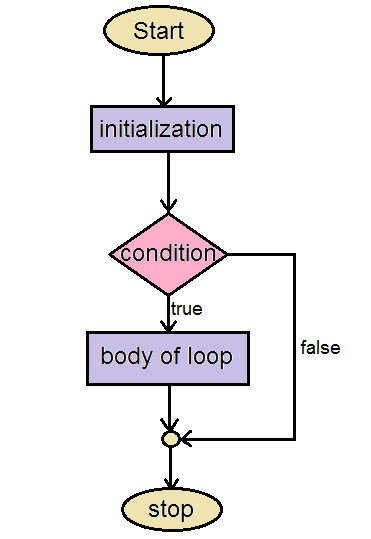
\includegraphics[height=0.7\textheight]{Figures/loop-flow-chart}
\caption{Anatomy of a looping mechanism.}
\end{figure}\end{minipage}}
\end{frame}
%
\section{\texttt{while} loops}
\begin{frame}{\texttt{while} loops}
\vfill
\begin{table}[]
\begin{flushleft}
\begin{tabular}{ll}
\texttt{while <condition>:} &  \\
\texttt{\qquad statement}        & \\
\texttt{\qquad statement}        & \\
\texttt{\qquad ...}        & \\
\texttt{\qquad statement}        & \\
\end{tabular}
\end{flushleft}
\end{table}
\vfill
\begin{itemize}
	\item \texttt{<condition>} evaluates to a Boolean (\texttt{True} or \texttt{False})
\end{itemize}
\begin{enumerate}
	\item if \texttt{<condition>} is \texttt{True}, then execute all statements inside the \texttt{while} block
	\item evaluate \texttt{<condition>} again
	\item repeat until \texttt{<condition>} is \texttt{False}
\end{enumerate}
\vfill
\end{frame}
%
\begin{frame}
\vfill
Example:
\begin{table}[]
\begin{flushleft}
\begin{tabular}{ll}
\texttt{n = input("You are in the Lost Forest. Go Left or Right?: ")} &  \\
\texttt{while n == "Right":}        & \\
\texttt{\qquad n = input("You are in the Lost Forest. Go Left or Right?: ")}        & \\
\texttt{print("You are out of the Lost Forest.")}        & \\
\end{tabular}
\end{flushleft}
\end{table}
\vfill
\end{frame}
%
\section{\texttt{for} loops}
\begin{frame}{\texttt{for} loops}
\vfill
\begin{table}[]
\begin{flushleft}
\begin{tabular}{ll}
\texttt{for <variable> in range(<number>):} &  \\
\texttt{\qquad statement}        & \\
\texttt{\qquad statement}        & \\
\texttt{\qquad ...}        & \\
\texttt{\qquad statement}        & \\
\end{tabular}
\end{flushleft}
\end{table}
\vfill
\begin{itemize}
	\item each time through the loop, \texttt{<variable>} takes some value
	\item \texttt{<variable>} starts from the smallest value (usually, \texttt{1})
	\item next time, \texttt{<variable> = <variable> + 1}
\end{itemize}
\vfill
\end{frame}
%
\subsection{the \texttt{range()} function}
\begin{frame}
\vfill
The \texttt{range(start,stop,step)} function returns a sequence of numbers, starting from \texttt{start}, and increments by \texttt{step}, and stops at \texttt{stop-1}.\\
Keep in mind the following caveats:
\begin{itemize}
	\item \texttt{stop} is mandatory
	\item \texttt{step} is optional: if not provided, it defaults to \texttt{1}
	\item \texttt{start} is optional: if not provided, it defaults to \texttt{0}
\end{itemize}
\vfill
Examples:
\begin{table}[]
\begin{flushleft}
\begin{tabular}{ll}
\texttt{mysum = 0} &  \\
\texttt{for i in range(7, 10):} &  \\
\texttt{\qquad mysum = mysum + i}        & \\
\texttt{print(mysum)}        & \\
\end{tabular}
\end{flushleft}
\end{table}
\begin{table}[]
\begin{flushleft}
\begin{tabular}{ll}
\texttt{mysum = 0} &  \\
\texttt{for i in range(5, 11, 2):} &  \\
\texttt{\qquad mysum = mysum + i}        & \\
\texttt{print(mysum)}        & \\
\end{tabular}
\end{flushleft}
\end{table}
\vfill
\end{frame}
%
\section{\texttt{for} vs. \texttt{while} loops}
\begin{frame}{\texttt{for} vs. \texttt{while} loops}
\vfill
Iterate through sequence of numbers in $[0, 5)$:
\begin{table}[]
\begin{flushleft}
\begin{tabular}{ll}
\texttt{\# with while loop} &  \\
\texttt{n = 0} &  \\
\texttt{while n < 5:} &  \\
\texttt{\qquad print(n)}        & \\
\texttt{\qquad n = n + 1}        & \\
\end{tabular}
\end{flushleft}
\end{table}
\begin{table}[]
\begin{flushleft}
\begin{tabular}{ll}
\texttt{\# with for loop} &  \\
\texttt{for n in range(5):} &  \\
\texttt{\qquad print(n)}        & \\
\end{tabular}
\end{flushleft}
\end{table}
\vfill
\end{frame}
%
\begin{frame}
\vfill
\adjustbox{valign=t}{\begin{minipage}[t]{0.49\textwidth}
\texttt{for} loops:
\begin{itemize}
	\item \textcolor{red}{known} number of iterations
	\item can \textcolor{red}{end early} via \texttt{break}
	\item (natively) uses a \textcolor{red}{counter}
	\item you \textcolor{red}{can rewrite} a \texttt{for} loop using a \texttt{while} loop
\end{itemize}
\end{minipage}}%
\hfill
\adjustbox{valign=t}{\begin{minipage}[t]{0.49\textwidth}
\texttt{while} loops:
\begin{itemize}
	\item \textcolor{red}{unbounded} number of iterations
	\item can \textcolor{red}{end early} via \texttt{break}
	\item you can use a \textcolor{red}{counter}, but you must initialise it before the loop and increment it inside the loop
	\item you \textcolor{red}{may not be able to rewrite} a \texttt{while} loop using a \texttt{for} loop
\end{itemize}
\end{minipage}}
\vfill
\end{frame}
%
\section{More on \texttt{for} loops}
\begin{frame}{More on \texttt{for} loops}
\vfill
\texttt{for} loops can be used to iterate over other data structures (e.g., lists or dictionaries\footnote{We will see lists and dictionaries later in the course}).
\vfill
Example: print all functions in the \texttt{math} module that contain the word `\texttt{log}'
\begin{table}[]
\begin{flushleft}
\begin{tabular}{ll}
\texttt{import math} &  \\
\texttt{for f in dir(math):} &  \\
\texttt{\qquad if 'log' in f:}        & \\
\texttt{\qquad\qquad print(f)}        & \\
\texttt{print("Done!")} &  \\
\end{tabular}
\end{flushleft}
\end{table}
\vfill
\begin{block}{Recall}
\texttt{dir()} returns a list.
\end{block}
\vfill
\end{frame}
%
\section{Nested Loops}
\begin{frame}{Nested Loops}
\vfill
We know that branching (i.e., \texttt{if}) statements can be arbitrarily nested. The same holds for loops.
\vfill
Example:
\begin{table}[]
\begin{flushleft}
\begin{tabular}{ll}
\texttt{mysum = 0} &  \\
\texttt{ } &  \\
\texttt{for i in range(3):} &  \\
\texttt{\qquad for x in range(2):}        & \\
\texttt{\qquad\qquad mysum += i}        & \\
\texttt{ } &  \\
\texttt{print(mysum)} &  \\
\end{tabular}
\end{flushleft}
\end{table}
\vfill
\begin{block}{Recall}
\texttt{mysum += i} is the same as \texttt{mysum = mysum + i}
\end{block}
\vfill
\end{frame}
%
\section{\texttt{break} statement}
\begin{frame}{\texttt{break} statement}
\vfill
The \texttt{break} statement:
\begin{itemize}
	\item immediately exits whatever loop is it in
	\item all further statements in the block are skipped
	\item exits only the innermost loop
	\item usually triggered at given condition
\end{itemize}
\vfill
\begin{table}[]
\begin{flushleft}
\begin{tabular}{ll}
\texttt{while <condition\_1>:} &  \\
\texttt{\qquad while <condition\_2>:} &  \\
\texttt{\qquad\qquad <statement\_a>}        & \\
\texttt{\qquad\qquad break}        & \\
\texttt{\qquad\qquad <statement\_b>}        & \\
\texttt{\qquad <statement\_c>}        & \\
\end{tabular}
\end{flushleft}
\end{table}
\vfill
%What's going on here?
%\vfill
\end{frame}
%
\begin{frame}
\vfill
Example:
\begin{table}[]
\begin{flushleft}
\begin{tabular}{ll}
\texttt{mysum = 0} &  \\
\texttt{ } &  \\
\texttt{for i in range(5, 11, 2):} &  \\
\texttt{\qquad mysum += i} &  \\
\texttt{\qquad if mysum == 5:}        & \\
\texttt{\qquad\qquad break}        & \\
\texttt{\qquad\qquad mysum += i} &  \\
\texttt{ } &  \\
\texttt{print(mysum)} &  \\
\end{tabular}
\end{flushleft}
\end{table}
\vfill
What's going on here?
\vfill
\end{frame}
%
\begin{frame}
\vfill
Nested loops with \texttt{break}, an example:
\begin{table}[]
\begin{flushleft}
\begin{tabular}{ll}
\texttt{mysum = 0} &  \\
\texttt{ } &  \\
\texttt{for i in range(30):} &  \\
\texttt{\qquad for n in range(20):} &  \\
\texttt{\qquad\qquad if n > 2:}        & \\
\texttt{\qquad\qquad\qquad break}        & \\
\texttt{\qquad\qquad mysum += i} &  \\
\texttt{\qquad if i>1:} &  \\
\texttt{\qquad\qquad break} &  \\
\texttt{ } &  \\
\texttt{print(mysum)} &  \\
\end{tabular}
\end{flushleft}
\end{table}
\vfill
What's going on here?
\vfill
\end{frame}
%------------------------------------------------------------------------------
% \section{Exercises}
% \begin{frame}{Exercises}
% \textcolor{red}{Exercise \#1: Coin flipping}
% \vspace{0.4cm}
% \begin{itemize}
% 	\item Ask the user how many coin tosses have to be performed
% 	\item Keep track of the number of times we get heads and tails
% 	\item We assume a \textit{fair coin} (i.e., unbiased 50\% change of getting head and tail at each toss)
% \end{itemize}
% %Ask the user how many coin tosses have to be performed.\\
% %Then, keep track of the number of times we get heads and tails.\\
% %We assume a \textit{fair coin} (i.e., unbiased 50\% change of getting head and tail at each toss).
% \begin{block}{Hint}
% You may use the \texttt{random.randint()} function to extract pseudo-random integers. To use it, \texttt{import} the \texttt{random} module.
% \end{block}
% \end{frame}
% %
% \begin{frame}%{Exercises}
% \textcolor{red}{Exercise \#2: Sum of sequence}\\
% \vspace{0.4cm}
% Write a function named \texttt{rolling\_sum()} that:
% \begin{itemize}
% 	\item repeatedly asks the user to insert a number
% 	\item we assume integer numbers
% 	\item keeps track of the sum of the numbers inserted so far
% 	\item if the user inserts $0$, then exit and return the sum
% \end{itemize}
% %\begin{block}{Hint}
% %You may use the \texttt{random.randint()} function to extract pseudo-random integers. To use it, \texttt{import} the \texttt{random} module.
% %\end{block}
% \end{frame}
% %
% \begin{frame}%{Exercises}
% %\textcolor{red}{Exercise \#3: Primality test}\\
% %\vspace{0.4cm}
% %Write a function that:
% %\begin{itemize}
% %	\item ask the user to insert an integer number, say $n$
% %	\item print on screen all prime numbers smaller than $n$
% %\end{itemize}
% %\begin{block}{Recall}
% %A \textit{prime} number is a natural number greater than 1 that has no positive divisors other than 1 and itself.
% %\end{block}
% %\begin{block}{Hint}
% %The simplest primality test aims at checking whether $n$ is evenly divisible (i.e., division with no remainder) by any number in range $[2, n/2]$. If so, the number is not prime.
% %\end{block}
% \textcolor{red}{Exercise \#3: Odd or even?}\\
% \vspace{0.4cm}
% Write a function named \texttt{odd\_or\_even()} that:
% \begin{itemize}
% 	\item accepts an integer number, say $n$
% 	\item prints the number of odd numbers in range $[1,n]$ (i.e., both included)
% 	\item prints the number of even numbers in range $[1,n]$ (i.e., both included)
% \end{itemize}
% \end{frame}
% %
% \begin{frame}%{Exercises}
% \textcolor{red}{Exercise \#4: The Fibonacci Sequence}\\
% \vspace{0.4cm}
% %Write a function that:
% %\begin{itemize}
% %	\item ask the user to insert a natural number, say $n$
% %	\item print all numbers $x$ and $y$ such that $x^2+y^2=z^2$, for any $z$
% %	\item perform the evaluation for all $x,y\leq n$
% %\end{itemize}
% %\begin{block}{Recall}
% %The Pythagorean triple consists of three positive integers $x$, $y$ and $n$, with $x,y \leq n$, such that:
% %\begin{equation*}
% %	x^2 + y^2 = n^2
% %\end{equation*}
% %\end{block}
% Write a function named \texttt{fibonacci1()} that:
% \begin{itemize}
% 	\item accepts an integer number, say $n$
% 	\item prints the first $n$ elements of the Fibonacci sequence.
% \end{itemize}
% \begin{block}{Definition}
% Each number in the Fibonacci sequence is given by the sum of the two preceding ones.\\
% The Fibonacci sequence starts with two `seed' numbers (\texttt{0} and \texttt{1}) and then the proper sequence starts:\\
% \qquad \texttt{0, 1, }\textcolor{blue}{1, 2, 3, 5, 8, 13, 21, ...}
% \end{block}
% \end{frame}
% %
% \begin{frame}%{Exercises}
% \textcolor{red}{Exercise \#5: The Fibonacci Sequence}\\
% \vspace{0.4cm}
% Write a function named \texttt{fibonacci2()} that:
% \begin{itemize}
% 	\item accepts an integer number, say $n$
% 	\item prints all Fibonacci numbers smaller than $n$.
% \end{itemize}
% \begin{block}{Definition}
% Each number in the Fibonacci sequence is given by the sum of the two preceding ones.\\
% The Fibonacci sequence starts with two `seed' numbers (\texttt{0} and \texttt{1}) and then the proper sequence starts:\\
% \qquad \texttt{0, 1, }\textcolor{blue}{1, 2, 3, 5, 8, 13, 21, ...}
% \end{block}
% \end{frame}
% %
% \begin{frame}%{Exercises}
% \textcolor{red}{Exercise \#6: Multiples}\\
% \vspace{0.4cm}
% Write a function named \texttt{multiples()} that:
% \begin{itemize}
% 	\item accepts an integer number, say $n$
% 	\item iterates the integers in $[1, n]$
% 	\item for multiples of 3, print \texttt{`Mult3'} instead of the number
% 	\item for multiples of 5, print \texttt{`Mult5'} instead of the number
% 	\item for multiples of 5 and 3, print \texttt{`Mult35'} instead of the number
% \end{itemize}
% \end{frame}
% %
% \begin{frame}%{Exercises}
% \textcolor{red}{Exercise \#7: Print a subset}\\
% \vspace{0.4cm}
% Write a function named \texttt{print\_subset()} that:
% \begin{itemize}
% 	\item accepts an integer number, say $n$
% 	\item accepts an integer number, say $m \leq n$
% 	\item scans all integer numbers in range $[1, n]$, but prints all numbers in range $[1, m]$
% \end{itemize}
% \end{frame}
%------------------------------------------------------------------------------
%\section{References}
%\begin{frame}[allowframebreaks]{References}
%%\bibliographystyle{apacite}
%\printbibliography[heading=none]
%\end{frame}
\section{References}
\begin{frame}{References}
\begin{itemize}
	\item Guttag, J. V. (2013). \textit{Introduction to Computation and Programming using Python (Revised and Expanded Edition)}. MIT Press. [Sections 2.4, 3.2]
	\item Downey, A. (2015). \textit{Think Python}. Green Tea Press ed. 2nd. [Sections 4.2, 7.3, 7.4]
\end{itemize}
\end{frame}
%------------------------------------------------------------------------------
\section{Acknowledgments}
\begin{frame}{Acknowledgments}
\begin{itemize}
	% \item Prof. Irene Finocchi (LUISS University)\\
	% \quad \textit{Introduction to Computer Programming} Lecture Notes (2020-2021)
	\item \url{https://www.codingeek.com/tutorials/c-programming/for-loop-in-c-programming-language-iteration-statements/}
	\item \url{https://docs.python.org/3/library/random.html}
\end{itemize}
\end{frame}
%------------------------------------------------------------------------------
%\subsection{Sites legais}
%\begin{frame}{Sites legais}
%  Want to know more? See!
%  \begin{itemize}
%    \item Browse in my page \url{http://www.ezefranca.com}.
%    \item Browse on BCC page \url{http://www.sp.senac.br/bcc}.
%    \item Thanks WriteLaTeX from Support! \url{http://www.writelatex.com}.
%  \end{itemize}
%
%\end{frame}
%------------------------------------------------------------------------------

% -----------------------------------------------------------------------------
\end{document}
%-----------------------------------------------Este comentario nunca aparecera
